\documentclass[11pt, letterpaper]{article}
\usepackage{amsmath} % Enhanced math support
\usepackage{amsfonts} % Additional math fonts
\usepackage{amssymb} % Additional math symbols
\usepackage{mathtools} % Additional tools for mathematical typesetting
\usepackage{bm} % Bold math symbols
\usepackage{physics} % Convenient macros for typesetting physics equations
\usepackage{siunitx} % Typesetting units and quantities
\usepackage{graphicx} % Enhanced support for graphics
\usepackage{hyperref} % Enhanced cross-referencing
\usepackage{cleveref} % Enhanced cross-referencing capabilities
\usepackage{enumerate} % Customizable enumeration
\usepackage{enumitem} % Enhanced enumeration
\usepackage{listings} % Typesetting source code
\usepackage{algorithm} % Typesetting algorithms
\usepackage{algpseudocode} % Typesetting pseudocode
\usepackage{float} % Improved interface for floating objects

\hypersetup{
    colorlinks=true,
    linkcolor=blue,
    filecolor=magenta,
    urlcolor=cyan,
}

\usepackage[left=1in, right=1in, top=1in, bottom=1in]{geometry}

\title{Predator and Prey Model Writeup}
\author{Mustafif Khan}
\date{April 5th, 2024}

\begin{document}
\maketitle
\newpage
\tableofcontents
\newpage
\pagenumbering{arabic}
\section{The Predator-Prey Model}
The Predator-Prey model is a mathematical model used to describe the
dynamics of two species in an ecosystem. The model consists of two first-order
non-linear differential equations that describe the interaction between the two
species. The model is also known as the Lotka-Volterra model and looks like the
following:

\begin{align}
    \frac{dx}{dt} & = ax - bxy = x(a-by)     \\
    \frac{dy}{dt} & = -cy + exy = y(-c + ex)
\end{align}

where $a$, $b$, $c$, and $e$ are $\geq 0$. The parameters have the
following meanings:

\begin{itemize}
    \item $x$: the population of the prey species (e.g. rabbits)
    \item $y$: the population of the predator species (e.g. foxes)
    \item $a$: the natural growth rate of prey in the absence of predation
    \item $b$: the death rate per encounter of prey due to predation
    \item $c$: the natural death rate of the predator in the absence of
          prey
    \item $e$: the efficiency of turning predated prey into predator
          offspring
\end{itemize}

\section{Dimensionless Equations}
To simplify the stability analysis of the model, we can make the equations
dimensionless. We achieve this by introducing the following dimensionless
variables:

\begin{align*}
    u (\tau) = \cfrac{ex(t)}{c}  \\
    v (\tau) = -\cfrac{by(t)}{a} \\
    \tau = at
\end{align*}

Substituting these variables into the original equations, we get the
following dimensionless equations:
\begin{align}
    \cfrac{du}{d\tau} & = u(1 - v)      \\
    \cfrac{dv}{d\tau} & = \alpha v(u-1)
\end{align}
Where $\alpha = \cfrac[diagonal]{c}{a}$.

\section{Equilibrium Points}
The equilibrium points of the system are found by setting the right hand
side of the equations to zero. This gives us the following equilibrium
points, $(0, 0)$ and $(1, 1)$.

\noindent The Jacobian matrix of the system is given by:
\begin{align*}
    J(u, v) = \begin{bmatrix}
                  1-v      & -u          \\
                  \alpha v & \alpha(u-1)
              \end{bmatrix}
\end{align*}

The eigenvalues of the Jacobian matrix at the equilibrium points are

\begin{align*}
    J(0, 0) = \begin{bmatrix}
                  1 & 0       \\
                  0 & -\alpha
              \end{bmatrix} \\
\end{align*}
\begin{align*}
    J(1, 1) = \begin{bmatrix}
                  0      & -1 \\
                  \alpha & 0
              \end{bmatrix}
\end{align*}

The eigenvalues of $J(0, 0)$ are $1$ and $-\alpha$, and the eigenvalues of
$J(1, 1)$ are $\pm i\sqrt{\alpha}$.

\section{Stability Analysis}

Since the eigenvalues of $J(0, 0)$ are both real and that $\lambda_1
    \lambda_2 < 0$, the equilibrium point $(0, 0)$ is a saddle point.
Since both of the eigenvalues of $J(1, 1)$ are complex, the equilibrium
point $(1, 1)$ is a center, or stable/unstable spiral.

\begin{itemize}
    \item The equilibrium point $(0, 0)$ represents when both species are
          extinct.
    \item The equilibrium point $(1, 1)$ represents when both species coexist
          in time.
    \item A center can lead to a regular, cyclic behavior in both populations
          that oscillate around the equilibrium point in a stable manner.
    \item A stable spiral indicates that there can be a perturbation in one of
          the populations, but they will eventually return to the equilibrium
          state.
    \item An unstable spiral suggests that the populations can experience
          population collapses or rapid growth due to a small perturbation.
\end{itemize}

Consider the following example where we have the following values for the
parameters: $a = 0.1$, $b = 0.02$, $c = 0.2$, and $e = 0.01$. Then the
dimensionless
equations are as follows:

\begin{align*}
    \cfrac{du}{d\tau} & = u(1 - v) \\
    \cfrac{dv}{d\tau} & = 2v(u-1)
\end{align*}
This has the following Jacobian matrices at the equilibrium points:

\begin{align*}
    J(0, 0) = \begin{bmatrix}
                  1 & 0  \\
                  0 & -2
              \end{bmatrix}
    \quad
    J(1, 1) = \begin{bmatrix}
                  0 & -1 \\
                  2 & 0
              \end{bmatrix}
\end{align*}

The eigenvalues of $J(0, 0)$ are $1$ and $-2$, and has the following phase
plane analysis:
\begin{itemize}
    \item Trace = $1 - 2 = -1$
    \item Determinant = $1 \cdot -2 = -2$
    \item Discriminant = $(-1)^2 - 4(-2) = 1 + 8 = 9$
\end{itemize}

Since the discriminant is positive and the determinant is negative, the
equilibrium point $(0, 0)$ is a saddle point.

The Jacobian matrix at $(1, 1)$ has eigenvalues $\pm i\sqrt{2}$, and the phase
plane analysis is as follows:
\begin{itemize}
    \item Trace = $0$
    \item Determinant = $0 - (-2) = 2$
    \item Discriminant = $0^2 - 8 = -8$
\end{itemize}

Since the discriminant is negative and the trace is zero, the equilibrium point
$(1, 1)$ is a center. This is also justified by the phase-plane diagram below:
\begin{figure}[H]
    \centering
    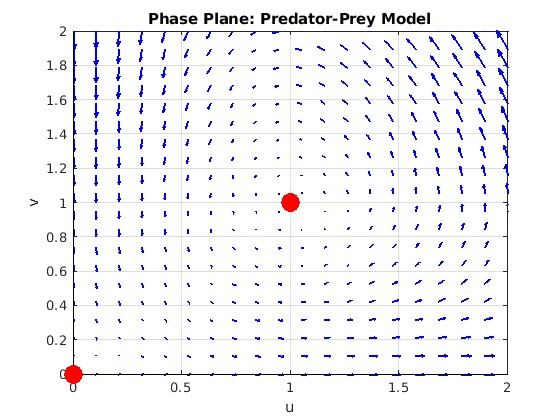
\includegraphics[width=0.8\textwidth]{plot.jpg}
    \caption{Phase Plane Diagram with $\alpha=2$}
\end{figure}
\end{document}
